\documentclass[tikz,border=8pt]{standalone}
% Shared look for every TikZ diagram. Load with \input{../../tools/tikz-style.tex}
\usepackage[T1]{fontenc}
\usepackage{lmodern}
\renewcommand{\sfdefault}{lmr}  % diagrams use the same serif as the text
\usetikzlibrary{arrows.meta, positioning, shapes.geometric, calc, fit, backgrounds}
\definecolor{cblue}{HTML}{4C78A8}
\definecolor{corange}{HTML}{F58518}
\definecolor{cgreen}{HTML}{54A24B}
\definecolor{cred}{HTML}{E45756}
\definecolor{cpurple}{HTML}{B279A2}
\definecolor{cgrey}{HTML}{6B6B6B}
\tikzset{
  every picture/.style={font=\sffamily, line width=1.2pt},
  box/.style={draw=#1, fill=#1!12, rounded corners=4pt, align=center, inner sep=7pt, minimum height=1.1cm},
  box/.default=cgrey,
  arrow/.style={-{Stealth[length=3mm]}, draw=cgrey, line width=1.4pt},
  title/.style={font=\sffamily\bfseries\Large},
  note/.style={font=\sffamily\small, text=cgrey, align=center},
}
\AtBeginDocument{\hyphenpenalty=10000 \exhyphenpenalty=10000}

\begin{document}
% Section 5: x_i = W_E[t_i] + W_P[i] for the first token, "Steve" (token 19206) at position 0. Learned weights in
% blue, data in grey (the Note's colour rule).
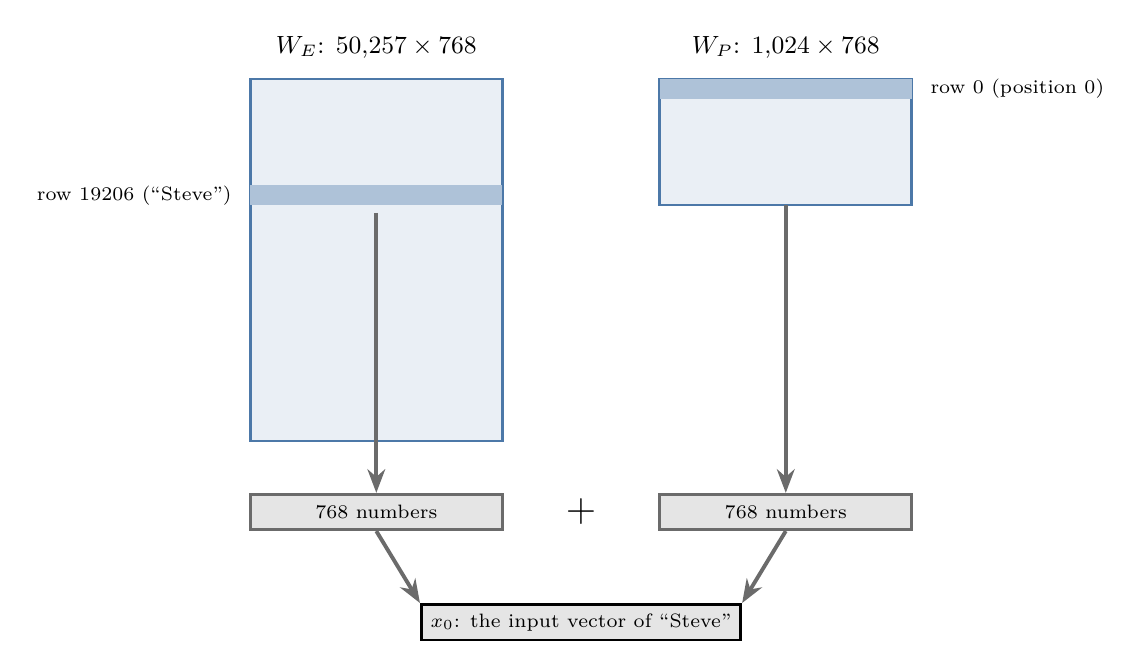
\begin{tikzpicture}[m/.style={draw=cblue, fill=cblue!12, line width=1pt, font=\sffamily\small, align=center},
  r/.style={draw=cblue, fill=cblue!45, line width=0.8pt}, v/.style={draw=cgrey, fill=black!10, line width=1pt, minimum width=3.2cm, minimum height=0.45cm, font=\sffamily\scriptsize}]
  \node[m, minimum width=3.2cm, minimum height=4.6cm] (WE) at (0, 0) {};
  \node[font=\sffamily\small, above=0.1cm of WE] {$W_E$: $50{,}257 \times 768$};
  \fill[cblue!45] (-1.6, 0.7) rectangle (1.6, 0.95);
  \node[font=\sffamily\scriptsize, anchor=east] at (-1.7, 0.82) {row 19206 (``Steve'')};
  \node[m, minimum width=3.2cm, minimum height=1.6cm] (WP) at (5.2, 1.5) {};
  \node[font=\sffamily\small, above=0.1cm of WP] {$W_P$: $1{,}024 \times 768$};
  \fill[cblue!45] (3.6, 2.05) rectangle (6.8, 2.3);
  \node[font=\sffamily\scriptsize, anchor=west] at (6.9, 2.17) {row 0 (position 0)};
  \node[v] (e) at (0, -3.2) {768 numbers};
  \draw[arrow] (0, 0.6) -- (e.north);
  \node[font=\sffamily\bfseries\Large] at (2.6, -3.2) {$+$};
  \node[v] (p2) at (5.2, -3.2) {768 numbers};
  \draw[arrow] (5.2, 0.7) -- (p2.north);
  \node[v, draw=black, minimum width=3.6cm] (x) at (2.6, -4.6) {$x_0$: the input vector of ``Steve''};
  \draw[arrow] (e.south) -- (x.north west); \draw[arrow] (p2.south) -- (x.north east);
\end{tikzpicture}
\end{document}
